\subsection{General Architecture}
\label{sec:CG-Architecture}

As many \IOT solutions, \IOTDSL massively relies on event processing. In order to transform abstract event definitions into runnable code, we rely on a middleware on which the event processing will run and that will be responsible for the evaluation of business rules. Figure~\ref{fig:gen-archi} depicts the general architecture of the \IOTDSL framework.

\begin{figure}%
	\centering  
	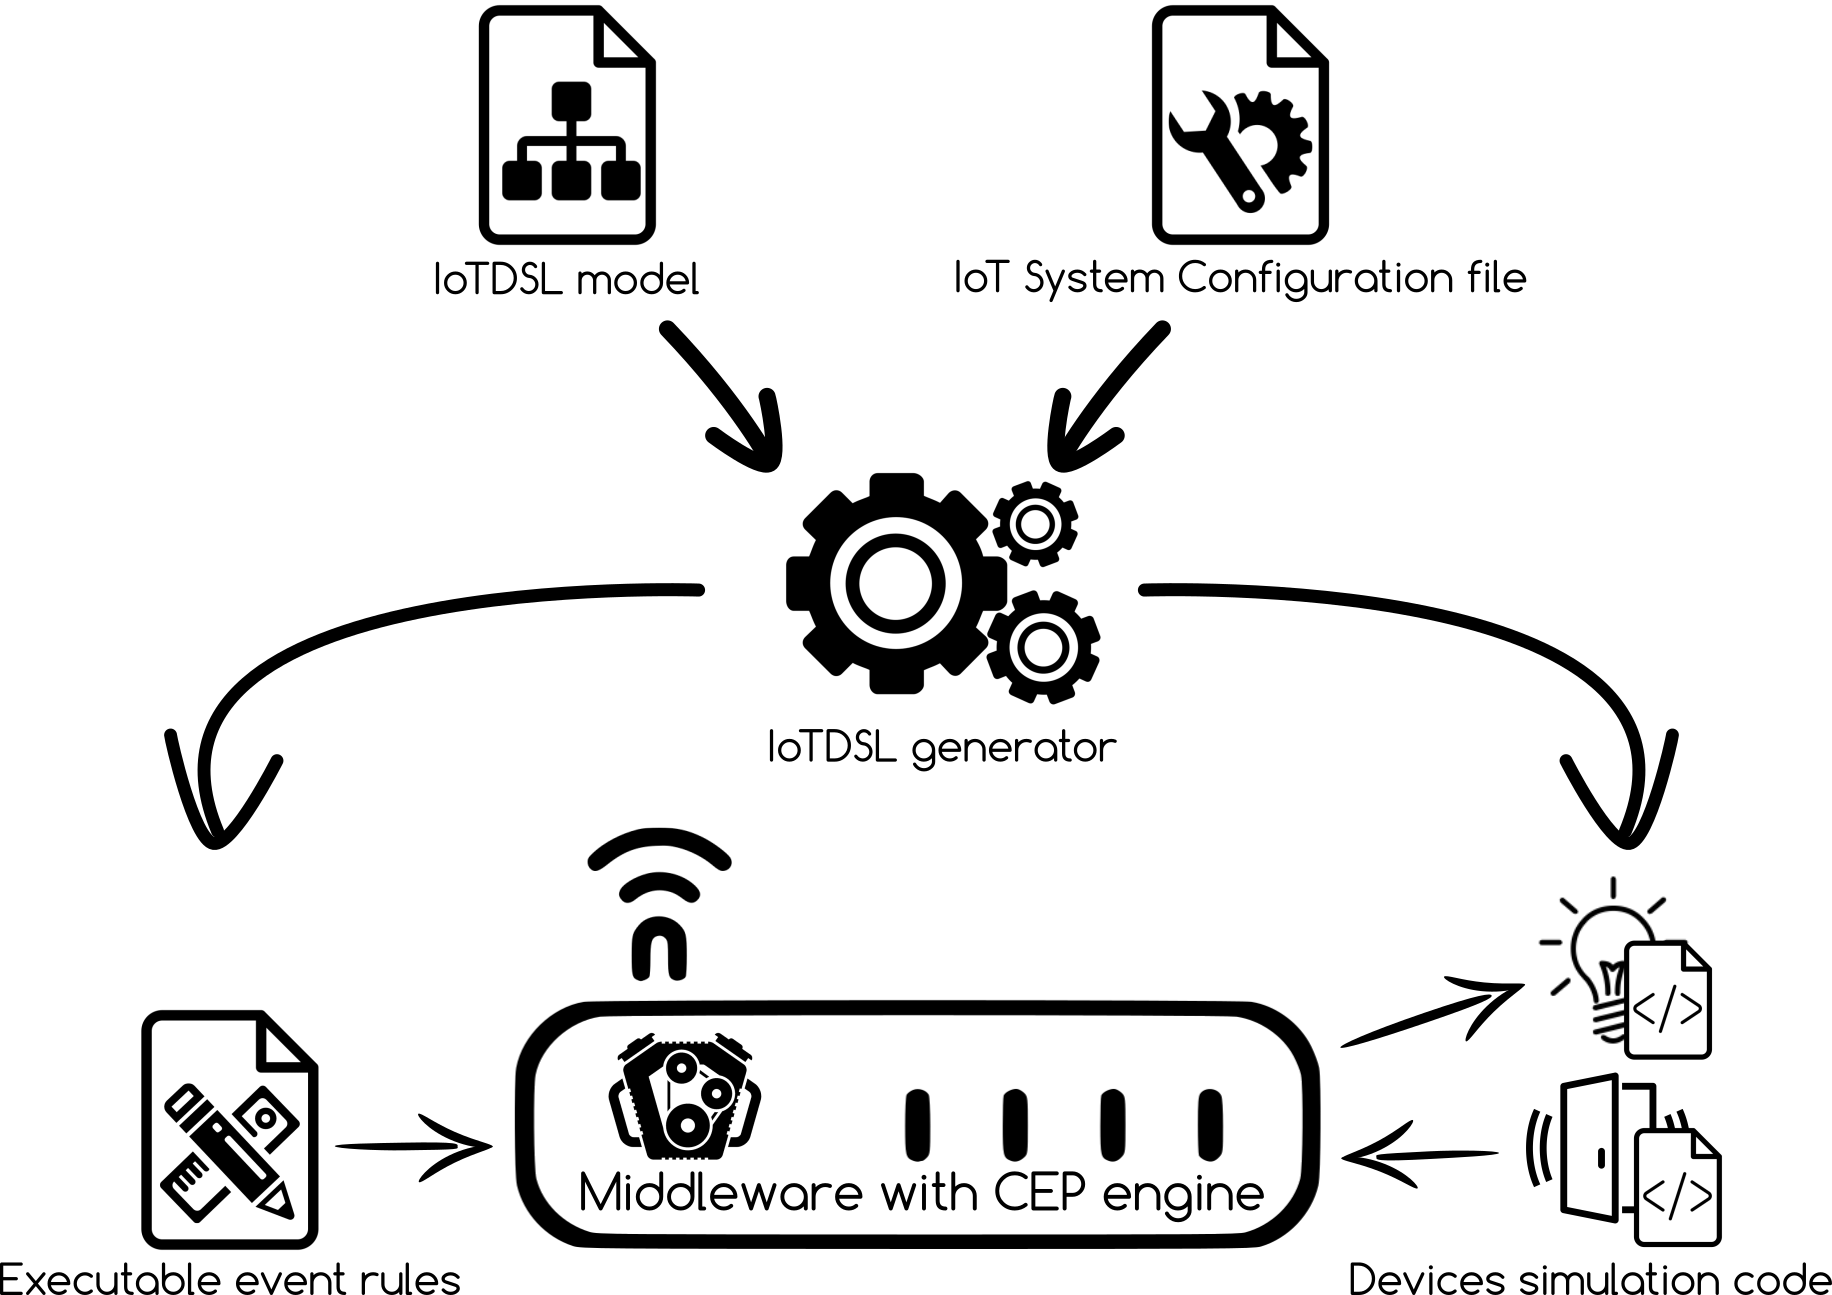
\includegraphics[width=.95\linewidth]{gen-archi.png}%
	\caption{General architecture of \IOTDSL framework}%
	\label{fig:gen-archi}%
\end{figure}

From \IOTDSL models, the generator will create a set of files that gather, on the one side, all rules as executable complex events and on the other side, a set of simulation code used to emulate the devices' behaviours. The event rules will be deployed in a \CEP engine running on a middleware and the individual simulation files will be used to test the whole infrastructure.

As we already mentioned, at present time the rules are all gathered and managed by a centralised entity where the simulation files are each emulating a single device. We are currently investigating how all business rules can be split into smaller chunks to be run on devices themselves when those objects have sufficient battery and CPU power. As we are developing the non-functional properties for \IOTDSL type and mapping definitions, those characteristics will be expressible in the form of technical specifications for devices and thus powerful equipments that are meeting some minimum requirements will be identified as deployment targets for distributed \CEP engines. 